\documentclass{article}
\usepackage{graphicx,fancyhdr,amsmath,amssymb,amsthm,subfigure,url,hyperref}
\usepackage[margin=1in]{geometry}
\usepackage{caption}
\usepackage{comment}
\usepackage{framed} 
\usepackage{indentfirst}
%\usepackage{supertabular,booktabs}
%\usepackage{supertabular}
%\usepackage{xtab}
\usepackage{amsmath}
\usepackage{csquotes}
\usepackage{longtable}
\usepackage{multicol}
\usepackage{appendix}
\setlength{\parindent}{1.5cm}

%------------ Algorithm Enviroment --------------
\usepackage{bbm}
\usepackage{algorithmic}
\usepackage[ruled,vlined]{algorithm2e}
%%%%%%
\SetKwProg{Fn}{Function}{}{}
%%%%%%

%------------ Bibliography  Setup --------------
\usepackage[english]{babel}
\usepackage[utf8]{inputenc}

%Includes "References" in the table of contents
\usepackage[nottoc]{tocbibind}

%------------ Hyperlinnk Setup --------------
\usepackage{hyperref}
\hypersetup{
    colorlinks=true,
    linkcolor=black,
    filecolor=magenta,      
    urlcolor=black,
    citecolor = black
}

% \hypersetup{
%     colorlinks=true,
%     linkcolor=blue,
%     filecolor=magenta,      
%     urlcolor=cyan,
% }
 
\urlstyle{same}

%--------------------------------- Tables ----------------------------------
\usepackage{multicol}
\usepackage{xtab}
\usepackage{booktabs}
\usepackage{array}
\usepackage[normalem]{ulem}
\useunder{\uline}{\ul}{}
\usepackage{floatrow}


\makeatletter
\let\mcnewpage\newpage
\newcommand{\changenewpage}{%
  \renewcommand\newpage{%
    \if@firstcolumn
      \hrule width\linewidth height0pt
      \columnbreak
    \else
      \mcnewpage
    \fi
}}
\makeatother

%----------------------- Macros and Definitions --------------------------




%%% FILL THIS OUT
\newcommand{\p}{\mathbb{P}}
\newcommand{\E}{\mathbb{E}}
%%% END
% Table float box with bottom caption, box width adjusted to content
\newfloatcommand{capbtabbox}{table}[][\FBwidth]

\newtheorem{theorem}{Theorem}



\renewcommand{\theenumi}{\bf \arabic{enumi}}

%\theoremstyle{plain}
%\newtheorem{theorem}{Theorem}
%\newtheorem{lemma}[theorem]{Lemma}

\fancypagestyle{plain}{}
\pagestyle{fancy}
\fancyhf{}
\fancyhead[RO,LE]{\sffamily\bfseries\large Stanford University}
\fancyhead[LO,RE]{\sffamily\bfseries\large CS230: Deep Learning}
%\fancyfoot[LO,RE]{\sffamily\bfseries\large \studentname: \suid @stanford.edu}
\fancyfoot[RO,LE]{\sffamily\bfseries\thepage}
\renewcommand{\headrulewidth}{1pt}
\renewcommand{\footrulewidth}{1pt}

\usepackage{float}
%\usepackage{subfig}
\graphicspath{{figures/}}


%-------------------------------- Title ----------------------------------

%\title{Deep Learning (CS230) Course Project Milestone}
\title{Hybrid Autoregressive-Recurrent Neural Network Architecture for Algorithmic Trading of Cryptocurrencies}
\author{
  Persson, Samuel\\
  \texttt{joelpe@stanford.edu}
  \and
  Slottje, Andrew\\
  \texttt{slottje@stanford.edu}
  \and
  Shaw, Ian\\
  \texttt{ieshaw@stanford.edu}
}

%--------------------------------- Text ----------------------------------
\begin{document}
\maketitle

\begin{abstract}
This investigation focuses on leveraging deep learning techiniques of cryptocurrency trading algorithms. We explore classic financial mathematics models of vector auto-regressive (VAR/VARMAX) and more complex recurrent neural networks (RNN) and a hybrid of the two in residual recurrent neural networks (R2N2). The find that the VAR model has phenomenal test period performance and thus props up the R2N2 model, while the RNN performs poorly. This implies that further investigation should focus on the best cost funcitons for neural network training for financial algorithms.
\end{abstract}

\section{Introduction and Literature Review}


Models used for time series prediction comprise one of the most important methods in economic forecasting. In particular, time series forecasting is important in the study of financial markets. Yet these models are frequently poorly performing, and accurate time-series forecasting is considered a `'top 10 problem" in data mining. \cite{YW} Moreover, markets tend to price in known information, and as a result it is difficult to discern any pattern in a market's movements without material nonpublic information. \cite{r} This is known as the "no arbitrage principle," and makes financial time series particularly vexing to predict.

While neural networks have been studied for applicability to time series data since at least the early 1990s, \cite{Azoff} many of these applications deal with contexts which are not subject to the no arbitrage principle (for example, forecasting crop yields or water levels) and do not experience the concomitant reduction of predictability in the data. A recent review of the literature is provided by Längkvist et al., who note applicability of techniques such as recurrent neural networks with LSTM. \cite{Lankvist} Logically, the long-term dependency recognition capacities that enable LSTM models to predict NLP outcomes with high success may translate to pattern recognition in the financial markets. It is well known, for instance, that cycles in the overall market are characterized by a particular geometry, with downturns exhibiting greater volatility in returns.

Previous research has noted the particular difficulty of forecasting cryptocurrency markets given their unusual volatility, and we look forward to accommodating this challenge. \cite{ian} To this end, we plan to implement RNN techniques, including RNN/LSTM learning on the residuals of vector autoregressive models, a hybrid method that has been successful in the literature. \cite{r2n2} We use Statsmodels and PyTorch for this purpose. 

We also hope to gain intuitive insight into the macrostructure of the cryptocurrency trading markets, enabling us to answer questions about capital flow into, out of, and within the cryptocurrency space. This exploration could add a quantitative voice to a conversation about the market which has been investigated from ecological \cite{ecology} and structural \cite{structure} perspectives. 

\section{Data}

On June 26, 2017 Rami Kawach, the founder of the crypto-currency exchange Bittrex, posted a link on twitter to a google drive containing price history data \cite{twitter_data}. These files log prices as they are updated, with granularity maxing out to one minute intervals. Each csv tracks the full history of each coin from ICO to June 25, 2017.

For our investigation, we use the hourly return against Bitcoin (BTC), volume, base volume, and spread for Ethereum (ETH), Litecoin (LTC), Ripple(XRP), Dash (DASH), and Monero (XMR). These coins were selected as they were the most liquid five currencies accross our data period of September 13, 2015 to June 25, 2017. 

For reference, Bittrex is incorporated and operated from the United States and maintains a New York Bitlicense. 

\subsection{Set Distributions}

To avoid bias with respect to the market regime, we split the data into a training set comprising September 2015 through December 2016, a cross-validation set comprising December 2016 through March 2017, and a test set comprising the remainder through June 2017. This equates to one year and one quarter (70\%), validated and tested on one quarter (15\%). Because time-dependent predictions should not incorporate future information, we do not partition the data randomly, as is typical in some other deep-learning applications.


\section{Models}


\subsection{Models}

\subsubsection{Multi-Coin Thesis}

Our exploration into multi-coin models (as opposed to a pure auto-regressive single asset approach) is base upon the thesis that of the five main coins there is a base amount of value that flows between the coins, and that there is some sort of leading-lagging dynamic amongst the high market-capitalization currencies. 

\subsubsection{Vector Auto-Regressive (VAR)}
Vector autoregression (VAR) is a method that models the discrete-time evolution of a stochastic variable $\omega_{t}$ as 
\[
\omega_{t}=\sum_{i=1}^{p} A_{i}\omega_{t-i}+c+\varepsilon_{t}\\
\]
where $A_{i}$ are a set of matrices expressing correlation in terms and $\varepsilon_{t}$ is the error term. As you can see, this model exposes linear relationships between trailing and upcoming data witht he hyperparameter of the lag $p$. 

We found through hyperparameter search acrross our validation set that the optimal lag for our setting is $p=1$, indicating a lag of a single time step, 1 hour. We believe this is works best due to the the high volatility of the cryptocurrency markets which do not allow for longer term linear relationships to develop. 

\subsubsection{Vector Auto-Regressive Moving Average Exogenous (VARMAX)}
The VARMAX model is an extension of the VAR model with the addition of moving average (MA) and exogenous (X) regressors. Our hyperparameter search found there to be no moving average predictability ($q=0$) so this will be left out of our discussion. The addiction of exogenous regressors is an investigation into external-market level factors that could shed further light into price movements. Common examples of exogenous factors are seasonaly or temporal phenomnenon. More specific examples could be how the US Stock Market may act erratically on monday mornings as traders hope to execute on the two days of weekend news that has been waiting to take effect. In short, exogenous factors are those that can have systematic effects onto the market while being outside the market. 

Mathematically, this takes the form of \cite{varmax}
\[
\omega_{t}=\sum_{i=1}^{p} A_{i}\omega_{t-i} + B x_t + c+\varepsilon_{t}\\
\]
Where we are fitting another matrix ($B$) of weights onto the feature vecotr $x_t$. Curiously, a hyperparameter search over our validation set found a $p=7$, seven hour time lag, to be optimal. This implies that the addition of exogenous feature attention allowed the model to see beyond the volatility that distracted the VAR model. 

\subsubsection{Multi-coin Recurrent Neural Network (RNN)}
The recurrent neural network approach attempts to leverage the power of long-short term memory (LSTM) architecture so that the network will learn for itelf the appropriate window from which to predict future returns.

Our investigation trained models with a stochastic gradient descent optimizer with 300 epoch passes throught the training set and a learning rate scheduler beginning at $0.01$ and shrinking by a factor of 10 twice through the trianing process.

We found through hyperparameter search that a network with ten hidden layers the following architecture to be optimal for our setting.

\[
\mathrm{Data}
\rightarrow \mathrm{Dense} 
\rightarrow \mathrm{LSTM}
\rightarrow \mathrm{LSTM}
\rightarrow\mathrm{Dense}
\rightarrow \mathrm{Prediction}
\]



\subsubsection{Multi-coin Residual Recurrent Neural Network (R2N2)}
The concept of a Residual Recurrent Neural Network was developed by Hardik et. al. with respect to error analysis \cite{r2n2}. The idea is essentially a form of feature engineeing, where a recurrent neural network does not learn the returns, but rather the residuals for an autoregressive model on the returns. 

Our investigation trained models with a stochastic gradient descent optimizer with 300 epoch passes throught the training set and a learning rate scheduler beginning at $0.01$ and shrinking by a factor of 10 twice through the trianing process.

We found through hyperparameter search that a network with ten hidden layers the following architecture to be optimal for our setting.

\begin{align*}
\mathrm{Data}
 \rightarrow  \mathrm{VAR} 
\rightarrow \mathrm{Dense}
\rightarrow \mathrm{ReLU} &
\rightarrow \mathrm{LSTM}
\rightarrow \mathrm{LSTM} \\
&\rightarrow \mathrm{LSTM}
\rightarrow \mathrm{LSTM}
\rightarrow \mathrm{LSTM}
\rightarrow \mathrm{LSTM}
\rightarrow\mathrm{Dense} + \mathrm{VAR} 
\rightarrow \mathrm{Prediction}
\end{align*}

Curiously, the R2N2 model necessitated many more LSTM layers for optimal MSE preformance which was still worse than that of the pure RNN. This is counter to the findings of Hardik et. al., where in their investigation the VAR feature engineering allowed the network to be shallower and quicker to learn a better prediction than the RNN. 

\section{Results}

For our results, we executed a backtest over the test set, without transaction costs included. The weigthing of any investment was done proportional to the predicted return, if a return was predicted to be 1.5, there would be a greter proportional investment than in assets where the return was predicted to be 0.5. If the predicted return was negative, no investment was made. At any given timestep, the entir eportfolio was allocated. 

\begin{center}
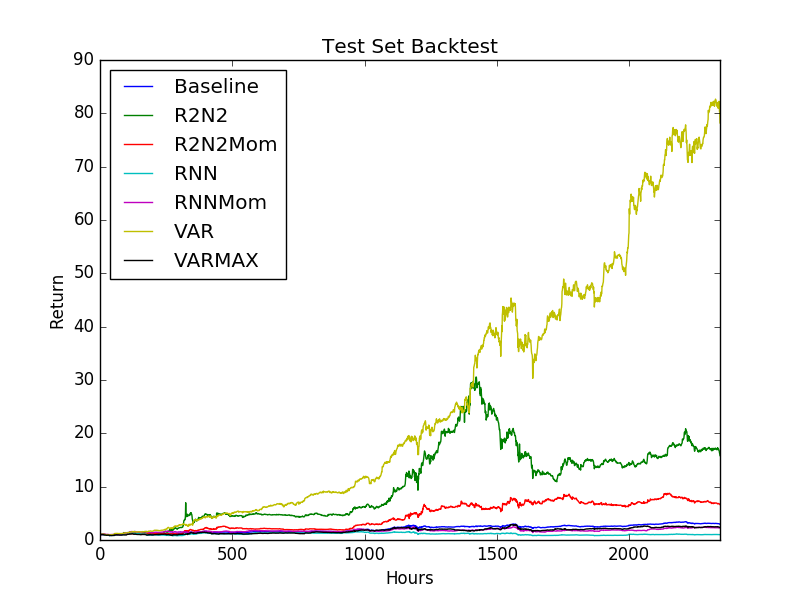
\includegraphics[scale = 0.6]{Results/backtest_all.png}
\end{center}

The visual of the backtest is seen in the figure above, and the results can be found in the table below.

\begin{tabular}{lrrrrr}
\toprule
{} &       auc &     return &    sharpe &       mse &  max\_drawdown \\
\midrule
Baseline &  0.500000 &   1.939799 &  2.886800 &  0.999415 &      0.292192 \\
R2N2     &  0.506587 &  14.827861 &  2.064562 &  0.000478 &      0.643012 \\
R2N2Mom  &  0.501317 &   5.641210 &  2.216578 &  0.000470 &      0.283592 \\
RNN      &  0.498271 &  -0.012393 & -0.067288 &  0.002232 &      0.490028 \\
RNNMom   &  0.501635 &   1.235352 &  4.249862 &  0.000472 &      0.437239 \\
VAR      &  0.542329 &  77.204319 &  3.145382 &  0.000472 &      0.332267 \\
VARMAX   &  0.498495 &   1.359462 &  2.640301 &  0.000478 &      0.442717 \\
\bottomrule
\end{tabular}




\section{Discussion}

\subsection{Observations}
The most obvious take away from the results is that none of our strategies beat the baseline. This is consistent with previous findings over the same dataset. \cite{ian} Yet, we believe this is also due to a difficulty in loss function and discerning metric (metric by which to compare models on the validation set) decisions. 

We also note that the R2N2 model outperforms the RNN. This gives creedence to the findings of Hardick et. al that the feeding of residuals can improve the RNN predicatbility. Thus between this, and the earlier findings of necessitating a deeper R2N2 for still worse MSE loss than the RNN, we will stay unresolved on the efficacy of the R2N2 model. 

\subsection{Discerning Metrics}

We included strategies trained with moentum coefficients (R2N2Mom, RNNMom) in our test set results. The reason is that even though they under-preformed those trained without momentumon the validation set, the experienced less variance between the training and test set returns. As you can see, this had mixed results on returns over the test set. 

This provides an interesting background into the difficulty of deciding metrics for out-of-sample returns. In our investigation, we ranked models due to their in-sample returns on the validation set. Furthermore, we used mean squared error on out loss function, which we show does not translate to returns directly. Furthermore, AUC (area under the receiever operating characteristic curve), which we used as a metric of classificaiton accuracy, does not translate directly to superior returns either. Thus, we believe, the best way to imporve results would be a dedicated investigation in the best cost function and discerning metric for cryptocurrency algorithms. 

\subsection{VAR and R2N2 Excessive Pefromance}

The returns of the VAR algorithm, and the R2N2 (built on top of VAR) are excessive to the point of unbelievable. Yet, their other metrics of MSE and AUC are not proportionally excessive. Further suprise is shown that a random walk approach of simply guessing the next return to be the same as the previous return results in a loss of 87\% of the portfolio over the test period. 

\section{Future Work}

Throughout our investigation we gained curiosity towards other lines of questioning; unfortunately the timeline of this project did not allow for the pursuit of all. In addition to what was mentioned at the end of the discussion section, here are our unpusued curiosities:

\begin{itemize}

	\item Exploring how training on narrower, more granular recent data effects model predicatibility. This could shed light on the speed of regime change for the cryptocurrency market.

	\item Classification prediction of positive or negative returns

	\item Multi-label Classificaiton of down a lot, down, up, up a lot

	\item Algorithmic allocation strategies for multi-coin signals

	\item VARMAX input into R2N2

	\item Explore use of normal feed forward networks, RNN-NARX, or CNN

	\item Explanatory investigation into what R2N2 is learning

	\item Predictive algorithms for volume so as to know when liquidity is sufficient for trades

	\item Explore relation of predictive accuracy to algorithm returns

	\item Signal with attention layer on top of RNN/R2N2

	\item Explore mini-batch learing options for financial time series data

\end{itemize}

\section{Contributions}
We apportioned work equally for the project. Joel worked on developing the VAR and VARMAX Models. Ian developed the multi-coin RNN and R2N2 models and constructed the backtester. Andrew worked with the literature review, data processing and the report.

\section{Codebase}
$\mathtt{https://github.com/ieshaw/deepcrypto.git}$
\bibliographystyle{unsrt}
\bibliography{refs}
\end{document}